\documentclass[12pt, twoside]{report}
\usepackage[a4paper,width=150mm,top=25mm,bottom=25mm,bindingoffset=6mm]{geometry}
\usepackage{graphicx}
\graphicspath{ {images/} }

\usepackage[english]{babel}
\usepackage[utf8]{inputenc}

\usepackage[style=alphabetic]{biblatex}
\addbibresource{references.bib}

\usepackage{fancyhdr}
\pagestyle{fancy}

\fancyhead{}
\fancyhead[RO,LE]{Thesis Title}
\fancyfoot{}
\fancyfoot[LE,RO]{\thepage}
\fancyfoot[LO,CE]{Chapter \thechapter}
\fancyfoot[CO,RE]{Felipe Balbi}

\renewcommand{\headrulewidth}{0.4pt}
\renewcommand{\footrulewidth}{0.4pt}

%% Define a \blankpage command that adds an empty page after current
\def\blankpage {
  \leavevmode
  \thispagestyle{empty}
  \newpage
}
%% Variables
%%
%% Customize the variables on variables.tex before continuing
\def \projectTitle    {Project Title}
\def \projectSubtitle {Project Subtitle}
\def \projectAuthor   {Author Name}
\def \projectDate     {\today}

\def \paperType       {a4paper}
\def \paperWidth      {150mm}
\def \marginTop       {25mm}
\def \marginBottom    {25mm}
\def \bindingOffset   {6mm}


%% Environment for a dedication page
\newenvironment{dedication}
               {
                 \clearpage            % we want a new page
                 \thispagestyle{empty} % no header and footer
                 \vspace*{\stretch{1}} % some space at the top 
                 \itshape              % the text is in italics
                 \centering            % text is centered
               }
               {
                 \par                    % end the paragraph
                 \vspace{\stretch{1}}  % space at bottom is the same as at the top
                 \clearpage            % finish off the page
               }

\title{\projectTitle}
\author{\projectAuthor}
\date{\projectDate}

\begin{document}

%% Frontmatter
%%
%% Change page numbering to lower case roman numerals
\pagenumbering{roman}
\begin{titlepage}
   \begin{center}
       \vspace*{1cm}

       \Huge
       \textbf{Project Title}

       \vspace{0.5cm}
       \Large
       Project Subtitle
            
       \vspace{1.5cm}

       \textbf{Author Name}

       \vfill
            
       A project report presented for the degree of\\
       Bachelor of Science in Computer Science
            
       \vspace{0.8cm}
     
       
\includegraphics[width=0.4\textwidth]{uol-arms.png}
            
       \Large
       Department Name\\
       Goldsmiths University of London\\
       UK\\
       21-12-2022
            
   \end{center}
\end{titlepage}

\blankpage
\thispagestyle{plain}
\begin{center}
    \Large
    \textbf{Thesis Title}
        
    \vspace{0.4cm}
    \large
    Thesis Subtitle
        
    \vspace{0.4cm}
    \textbf{Author Name}
       
    \vspace{0.9cm}
    \textbf{Abstract}
\end{center}
Lorem ipsum dolor...


\begin{scrdedication}
  To my family...
\end{scrdedication}


\chapter*{Declaration}
I declare that..


\chapter*{Acknowledgements}
I want to thank...



\tableofcontents
\listoffigures

%% Mainmatter
%%
%% Change page numbering to arabic numerals
\pagenumbering{arabic}
\chapter{Introduction}

\chapter{Chapter Two Title}


Lorem ipsum dolor
Lorem ipsum dolor
Lorem ipsum dolor
Lorem ipsum dolor
Lorem ipsum dolor
Lorem ipsum dolor
Lorem ipsum dolor
Lorem ipsum dolor
Lorem ipsum dolor
Lorem ipsum dolor
Lorem ipsum dolor
Lorem ipsum dolor
Lorem ipsum dolor
Lorem ipsum dolor
Lorem ipsum dolor
Lorem ipsum dolor
Lorem ipsum dolor
Lorem ipsum dolor
Lorem ipsum dolor
Lorem ipsum dolor
Lorem ipsum dolor
Lorem ipsum dolor
Lorem ipsum dolor
Lorem ipsum dolor
Lorem ipsum dolor
Lorem ipsum dolor
Lorem ipsum dolor
Lorem ipsum dolor
Lorem ipsum dolor
Lorem ipsum dolor
Lorem ipsum dolor
Lorem ipsum dolor
Lorem ipsum dolor
Lorem ipsum dolor
Lorem ipsum dolor
Lorem ipsum dolor
Lorem ipsum dolor
Lorem ipsum dolor
Lorem ipsum dolor
Lorem ipsum dolor
Lorem ipsum dolor
Lorem ipsum dolor
Lorem ipsum dolor
Lorem ipsum dolor
Lorem ipsum dolor
Lorem ipsum dolor
Lorem ipsum dolor
Lorem ipsum dolor
Lorem ipsum dolor
Lorem ipsum dolor
Lorem ipsum dolor
Lorem ipsum dolor
Lorem ipsum dolor
Lorem ipsum dolor
Lorem ipsum dolor
Lorem ipsum dolor
Lorem ipsum dolor
Lorem ipsum dolor
Lorem ipsum dolor
Lorem ipsum dolor
Lorem ipsum dolor
Lorem ipsum dolor
Lorem ipsum dolor
Lorem ipsum dolor
Lorem ipsum dolor
Lorem ipsum dolor
Lorem ipsum dolor
Lorem ipsum dolor
Lorem ipsum dolor
Lorem ipsum dolor
Lorem ipsum dolor
Lorem ipsum dolor
Lorem ipsum dolor
Lorem ipsum dolor
Lorem ipsum dolor
Lorem ipsum dolor
Lorem ipsum dolor
Lorem ipsum dolor
Lorem ipsum dolor
Lorem ipsum dolor
Lorem ipsum dolor
Lorem ipsum dolor
Lorem ipsum dolor
Lorem ipsum dolor
Lorem ipsum dolor
Lorem ipsum dolor
Lorem ipsum dolor
Lorem ipsum dolor
Lorem ipsum dolor
Lorem ipsum dolor
Lorem ipsum dolor
Lorem ipsum dolor
Lorem ipsum dolor
Lorem ipsum dolor
Lorem ipsum dolor
Lorem ipsum dolor
Lorem ipsum dolor
Lorem ipsum dolor
Lorem ipsum dolor
Lorem ipsum dolor
Lorem ipsum dolor
Lorem ipsum dolor
Lorem ipsum dolor
Lorem ipsum dolor
Lorem ipsum dolor
Lorem ipsum dolor
Lorem ipsum dolor
Lorem ipsum dolor
Lorem ipsum dolor
Lorem ipsum dolor
Lorem ipsum dolor
Lorem ipsum dolor
Lorem ipsum dolor
Lorem ipsum dolor
Lorem ipsum dolor
Lorem ipsum dolor
Lorem ipsum dolor
Lorem ipsum dolor
Lorem ipsum dolor
Lorem ipsum dolor
Lorem ipsum dolor
Lorem ipsum dolor
Lorem ipsum dolor
Lorem ipsum dolor
Lorem ipsum dolor
Lorem ipsum dolor
Lorem ipsum dolor
Lorem ipsum dolor
Lorem ipsum dolor
Lorem ipsum dolor
Lorem ipsum dolor
Lorem ipsum dolor
Lorem ipsum dolor
Lorem ipsum dolor
Lorem ipsum dolor
Lorem ipsum dolor
Lorem ipsum dolor
Lorem ipsum dolor
Lorem ipsum dolor
Lorem ipsum dolor
Lorem ipsum dolor
Lorem ipsum dolor
Lorem ipsum dolor
Lorem ipsum dolor
Lorem ipsum dolor
Lorem ipsum dolor
Lorem ipsum dolor
Lorem ipsum dolor
Lorem ipsum dolor
Lorem ipsum dolor
Lorem ipsum dolor
Lorem ipsum dolor
Lorem ipsum dolor
Lorem ipsum dolor
Lorem ipsum dolor
Lorem ipsum dolor
Lorem ipsum dolor
Lorem ipsum dolor
Lorem ipsum dolor
Lorem ipsum dolor
Lorem ipsum dolor
Lorem ipsum dolor
Lorem ipsum dolor
Lorem ipsum dolor
Lorem ipsum dolor
Lorem ipsum dolor
Lorem ipsum dolor
Lorem ipsum dolor
Lorem ipsum dolor
Lorem ipsum dolor
Lorem ipsum dolor
Lorem ipsum dolor
Lorem ipsum dolor
Lorem ipsum dolor
Lorem ipsum dolor
Lorem ipsum dolor
Lorem ipsum dolor
Lorem ipsum dolor
Lorem ipsum dolor
Lorem ipsum dolor
Lorem ipsum dolor
Lorem ipsum dolor
Lorem ipsum dolor
Lorem ipsum dolor
Lorem ipsum dolor
Lorem ipsum dolor
Lorem ipsum dolor
Lorem ipsum dolor
Lorem ipsum dolor
Lorem ipsum dolor
Lorem ipsum dolor
Lorem ipsum dolor
Lorem ipsum dolor
Lorem ipsum dolor
Lorem ipsum dolor
Lorem ipsum dolor
Lorem ipsum dolor
Lorem ipsum dolor
Lorem ipsum dolor
Lorem ipsum dolor
Lorem ipsum dolor
Lorem ipsum dolor
Lorem ipsum dolor
Lorem ipsum dolor
Lorem ipsum dolor
Lorem ipsum dolor
Lorem ipsum dolor
Lorem ipsum dolor
Lorem ipsum dolor
Lorem ipsum dolor
Lorem ipsum dolor
Lorem ipsum dolor
Lorem ipsum dolor
Lorem ipsum dolor
Lorem ipsum dolor
Lorem ipsum dolor
Lorem ipsum dolor
Lorem ipsum dolor
Lorem ipsum dolor
Lorem ipsum dolor
Lorem ipsum dolor
Lorem ipsum dolor
Lorem ipsum dolor
Lorem ipsum dolor
Lorem ipsum dolor
Lorem ipsum dolor
Lorem ipsum dolor
Lorem ipsum dolor
Lorem ipsum dolor
Lorem ipsum dolor
Lorem ipsum dolor
Lorem ipsum dolor
Lorem ipsum dolor
Lorem ipsum dolor
Lorem ipsum dolor
Lorem ipsum dolor
Lorem ipsum dolor
Lorem ipsum dolor
Lorem ipsum dolor
Lorem ipsum dolor
Lorem ipsum dolor
Lorem ipsum dolor
Lorem ipsum dolor
Lorem ipsum dolor
Lorem ipsum dolor
Lorem ipsum dolor
Lorem ipsum dolor
Lorem ipsum dolor
Lorem ipsum dolor
Lorem ipsum dolor
Lorem ipsum dolor
Lorem ipsum dolor
Lorem ipsum dolor
Lorem ipsum dolor
Lorem ipsum dolor
Lorem ipsum dolor
Lorem ipsum dolor
Lorem ipsum dolor
Lorem ipsum dolor
Lorem ipsum dolor

\documentclass[../main]{subfiles}

\begin{document}
\chapter{Chapter Three Title}

\lipsum[1-20]

Foooo \cite{einstein}

Baaaarrr \cite{knuthwebsite}

Bazzzz \cite{latexcompanion}

TEXT\parencite[see][p10]{latexcompanion}
TEXT\parencite[compare][]{knuthwebsite}
TEXT\parencite[e.g.][page 300]{einstein}
\end{document}

\chapter{Chapter Four Title}

\section{Typesetting Algorithms}

We can use the \emph{algorithm2e} package to typeset algorithm blocks in a way
that is pleasant to read. In listing \ref{alg:linear-search} we have an example
of a linear search algorithm typeset with \emph{algorithm2e}

\begin{function}[H]
  \For{$i \gets 0$ \KwTo $N$}{
    \If{$A[i] = e$} {
      \Return{true}
    }
  }
  \Return{false}
  \caption{LinearSearch($A,N,e$)}
  \label{alg:linear-search}
\end{function}

\section{Pictures are possible with TiKZ}

Any \LaTeX wouldn't be complete without an image drawn with TiKZ. Figure
\ref{fig:linear-search} shows the linear behavior of the Linear Search
algorithm.

\begin{figure}[h]
  \centering
  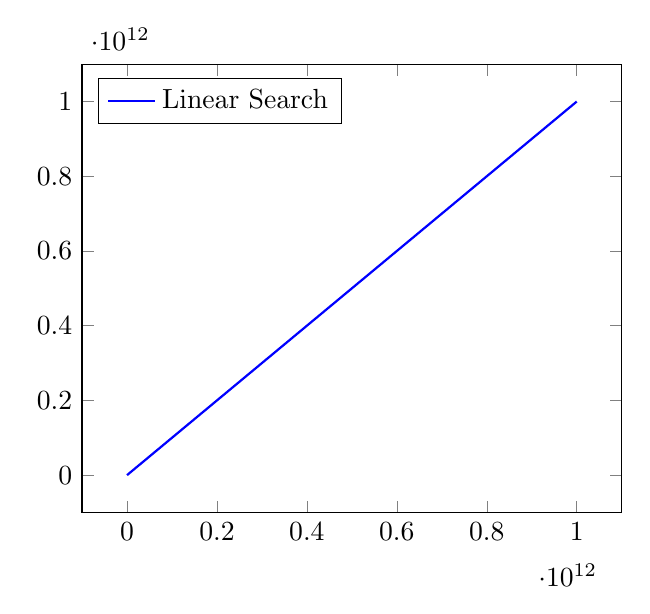
\begin{tikzpicture}
    \begin{axis}[
        legend pos=north west,
        legend cell align=left]
      \addplot[blue, thick, domain=1:1e12] {
        x
      };
      \addlegendentry{Linear Search};
    \end{axis}
  \end{tikzpicture}
  \caption{Linear Search Time Complexity}
  \label{fig:linear-search}
\end{figure}


\chapter{Conclusion}


%% Appendix
\appendix
\chapter{Appendix Title}


%% Backmatter
\printbibliography

\end{document}
